%%%%% Document Setup %%%%%%%%

\documentclass[12pt, onecolumn]{revtex4}    % Font size (12pt) and column number (one or two).

\usepackage{times}                          % Times New Roman font type

\usepackage[a4paper, left=2.5cm, right=2.5cm,
 top=2.5cm, bottom=2.5cm]{geometry}       % Defines paper size and margin length

\renewcommand{\baselinestretch}{1.15}     % Defines the line spacing

\usepackage[font=small,
labelfont=bf]{caption}                      % Defines caption font size and caption title bolded

\usepackage{graphics,graphicx,epsfig,ulem}	% Makes sure all graphics works
\usepackage{amsmath, amssymb} 						% Adds mathematical features for equations
\usepackage[compat=1.0.0]{tikz-feynman}
\usepackage{braket}
\usepackage{booktabs}

\usepackage{etoolbox}                       % Customise date to preferred format
\makeatletter
\patchcmd{\frontmatter@RRAP@format}{(}{}{}{}
\patchcmd{\frontmatter@RRAP@format}{)}{}{}{}
\renewcommand\Dated@name{}
\makeatother

\usepackage{fancyhdr}


\pagestyle{fancy}                           % Insert header
\renewcommand{\headrulewidth}{0pt}
\lhead{\small Dominic Robson}                          % Your name
\rhead{\small Umbrella Sampling and Pulling Simulations of two Protein Structures}            % Your report title               

\def\thesection{\arabic{section}}

\def\bibsection{\section*{References}}        % Position reference section correctly

\newcommand{\sgn}{\text{sgn}}

%%%%% Document %%%%%
\begin{document}                     


\title{Umbrella Sampling and Pulling Simulations of two Protein Structures} 
\date{Submitted: \today{}}
\author{Dominic Robson}
\affiliation{\normalfont King's College London}


\begin{abstract}              

Pulling and umbrella sampling simulations were performed on two simple protein structures, a helix and a hairpin.  Discontinuities were found in the PMFs and an attempt was made to explain this as coinciding with a lack of overlap of histograms in those regions.  The radius of gyration and end to end distance was calculated during the pulling simulations of the helix and it was shown that an ideal chain is not an appropriate model for the system that was considered.

\end{abstract}

\maketitle
%\thispagestyle{plain} % produces page number for front page

\tableofcontents

\newpage

\section{Introduction}

The configuration and behaviour of a protein under mechanical stress plays a key role in the behaviour of that protein\cite{StretchWhy}.  Therefore the study of how proteins behave when they are stretched or pulled is an extremely important area of investigation.\\

Biological proteins often have large and complex structures but often feature more simple building blocks including $\alpha$-helices and $\beta$-hairpins\cite{Chig}.  By studying the properties of such simple structures one can then hope to uncover information about more complex systems which are biologically relevant.\\

It is possible to strain proteins in the laboratory and determine the forces required for various kinds of deformation however relating these results to the energy profile of a system is extremely difficult\cite{MDWhy}.  Molecular dynamics simulations are therefore often used to simulate stresses being exerted on a protein in order to draw out such information\cite{MDWhy}.\\

In this report we will describe and analyse the results of simulations performed on simple helix and hairpin structures.  In section 2 we will outline some of the aspects of the umbrella sampling method for calculating the energy along a certain coordinate of the system.  In section 3 we will describe the structures that were simulated and the nature of the simulations performed.  The results of the simulations will be shown and discussed in section 4.   

\section{Umbrella Sampling, WHAM and Bootstrapping}

In this section we review the technique of Umbrella Sampling, how it can be used to infer the energy landscape of a molecule and how the uncertainty in such a calculation can be approximated.\\

One major purpose of biochemical molecular dynamics simulations is to uncover the free energy landscape of a molecule\cite{Umbrella}.  In particular one is often interested in the free energy differences between configurations of a molecule in which case, one usually defines some \textit{reaction coordinate}, a continuous parameter of the system for which the two desired configurations are easily distinguishable\cite{Umbrella}.  For a given system and desired configurations there could be many such reaction coordinates some of which may be more informative than others.  Choosing the reaction coordinate then requires some insight into the processes at work in the system\cite{Umbrella}.  In principle (provided ergodicity holds) the probability distribution of the system having a particular value of reaction coordinate $\xi$ can be well estimated by running the simulation for a long time and counting the number of occurrences of the system at $\xi$ \cite{GWHAM}.  However, most molecules have a complex free energy landscape with many local minima separated by potential barriers.  In an unbiased simulation the regions close to a local minimum will be extremely well sampled while those regions that are far from minima will be dramatically undersampled\cite{Umbrella} \cite{GWHAM}.  This makes the calculation of the free energy landscape along the entire reaction coordinate impossible.\\

One solution to the problem of undersampling of regions far from local minima is the use of \textit{umbrella sampling}\cite{Umbrella}.  The basic premise of this method is that one can add an additional potential which biases the system to remain close to a desired value of the reaction coordinate.  Many simulations can be run with different biasing potentials such that the entirety of phase space along the reaction coordinate is explored and not merely those areas close to energy minima\cite{Umbrella}.  Most commonly the bias potentials which are added take a harmonic form, each centred around a value $\xi_i$ where the index $i$ denotes the $i$-th simulation or \textit{window}\cite{GWHAM}.  Providing sufficient overlap of the different windows then the entire range of the reaction coordinate can be sampled well enough to derive the potential of mean force (PMF)\cite{GWHAM}.  The PMF and free energy of a system are identical up to a potential Jacobian factor dependent upon the choice of reaction coordinate\cite{PMF}.  Due to the biasing potentials however, the task of inferring the PMF from the probability distribution derived from the simulation is not straight forward and additional techniques are required.

\subsection{WHAM}

One method for deriving the PMF from an umbrella sampling simulation is the \textit{Weighted Histogram Analysis Method} (WHAM)\cite{Umbrella}\cite{GWHAM}.  The method works by finding the maximum likelihood estimate of the unbiased probability distribution and using this to infer the free energy.\\

Denoting by $N_w$ the number of umbrella sampling windows (simulation), each of which has an harmonic bias potential  $w_i (\xi) = 1/2 K_i (\xi - \xi_i)^2$ $ i = 1, 2,... N_w$, by $h_i(\xi)$ the histogram of reaction coordinates in that simulation and by $n_j$ the total number of sampled data in window $i$ then so-called WHAM equations are\cite{GWHAM}

\begin{align} 
\label{eq: WHAM}
P(\xi) &= \frac{\sum_{i =1}^{N_w}g_i ^{-1} h_i (\xi)}{\sum_{j =1}^{N_w} n_j g_j^{-1} e^{- \beta (w_j (\xi) - f_j)}}\\
e^{-\beta f_j} &= \int d \xi e^{-\beta w_j(\xi)} P(\xi) \equiv \mathbb{E} _\xi\left[e^{-\beta w_j(\xi)} \right].
\end{align}

In which we have also defined the inefficiency $g_j = 1 + 2 \tau_i$ where $\tau_i$ is the autocorrelation time \cite{GWHAM} of the system in window $i$, these terms will cancel if $\tau_i$ is the same in every window.  The WHAM equations are a pair of coupled equations which can be solved iteratively \cite{GWHAM}to find the free energy constants $f_i$ and the unbiased probability distribution $P(\xi)$.  Once the solutions have converged then the PMF can be calculated in reference to some point $\xi_0$ as PMF$(\xi) = - 1/\beta \log(P(\xi)/P(\xi_o))$\cite{GWHAM}.  In order to calculate the statistical uncertainty involved in this calculation, one possible method is \textit{bootstrapping}\cite{GWHAM}.

\subsection{Bootstrapping}

Bootstrapping is a powerful method for estimating the statistical uncertainty of a result derived from a large number of observations of a variable\cite{GWHAM}.  Using the observed values one can estimate the probability distribution for that variable.  Having obtained the probability distribution one then draws new samples of the variable at random according to the distribution and for each of these recalculates the desired result.  Repeating this process one can generate a large number of results and calculate the standard deviation to estimate the uncertainty.\cite{GWHAM}\\

In the case of umbrella sampling, in each sampling simulation the histogram of positions $h_i(\xi)$ results from a large number ($n_i$) of observations of $\xi$ and can be therefore used to estimate the probability distribution of $\xi$ within that window.  One is able to then draw samples of $xi$ from this derived distribution and for each sample recalculate the PMF\cite{GWHAM}.  After many such samples have been drawn and their PMF calculated the uncertainty in the PMF can then be approximated by standard deviation of ensemble of bootstrapped values.\\

Due to potentially long autocorrelation times, problems can arise in bootstrapping separately within the individual umbrella histograms resulting in a possibly large underestimate of the uncertainty\cite{GWHAM}.  One proposed means of avoiding this is known as Bayesian bootstrapping \cite{GWHAM}in which the bootstrapping is performed on the entire (complete) histograms and not the points within the individual histograms.  In addition each histogram $i$ is selected with a weighted probability $\omega_i$, during each bootstrap iteration a random set of weights is generated and assigned to the histograms.  In other words the complete distribution of $xi$ is treated as a probability mixture with each histogram selected with a random weight.  The probability of a histogram having a weight of zero is extremely small and therefore the probability of multiple histograms having close to zero weights is negligible.  Therefore as long as the histograms overlap sufficiently Bayesian bootstrapping should ensure complete sampling over the entire range of the reaction coordinate\cite{GWHAM}.  With the random weights the $g_i ^ {-1}$ terms in the WHAM equations (equation \ref{eq: WHAM}) must be replaced by $\omega_i g_i ^ {-1}$ in order to derive the PMF\cite{GWHAM}.  For both of our systems described in section 3 umbrella sampling simulations were carried out, the PMFs calculated along a certain reaction coordinate and, the uncertainty calculated using Bayesian bootstrapping.  The results will be shown in section 4.

\section{Structures and Simulation Methods}

In this section we outline the nature of the structures which have been simulated.  We also describe the nature of the simulations that were carried out. 

\subsection{Structures and Equilibration}

We begin by first briefly summarising the structure of the proteins to be simulated as well as giving some details about the initial set up of the systems.

\subsubsection{$\alpha$ - helix}

The $\alpha$-helix we will be looking at consists of 13 residues: LEU, GLN, LYS, TRP, GLN, GLN, PHE, ASN, SER, ASP, LEU, ASN, SER.\\

All simulations were performed using GROMACS\cite{GMX}.  The GROMOS96 53a6 force field\cite{FF}.  During the initial set up the helix was centred and aligned along the $z$-axis, water was then added as a solvent and energy minimisation and equilibration were then performed.\\

The minimisation was performed using a steepest descent algorithm\cite{GMX} which was terminated when the maximum force (i.e. the gradient) no longer exceeded 1000 kJ mol$^{-1}$ nm$^{-1}$.  We show the energy minimisation profile below in figure 1\\

\begin{figure}[h!]
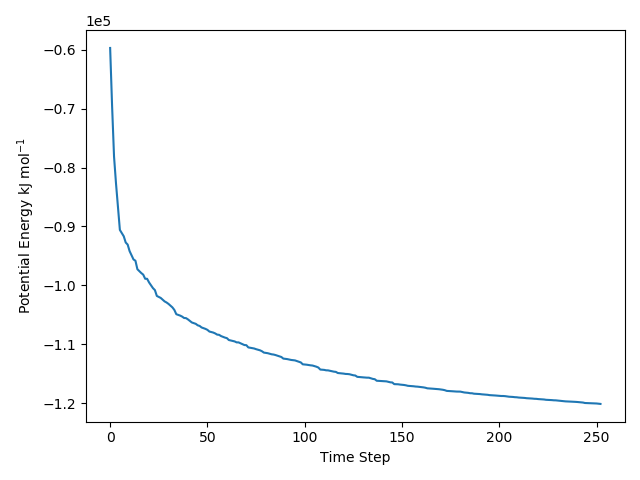
\includegraphics[scale=0.4]{HelixMin}
\caption{Potential energy profile of the helix during the energy minimisation procedure.}
\end{figure}

The system was then equilibrated under an NPT ensemble \cite{GMX} (constant particle number, pressure and temperature) in order to complete the set up.  Temperature and pressure coupling were performed using a Berensden-thermostat\cite{Ber}.  A leap-frog algorithm \cite{GMX} was used for solving the equations of motion and the reference temperature and pressure for the equilibration were 310K and 1.0 bar.   We show the pressure and temperature profiles below (figure 2), in both cases the system appears to have stabilised around the desired values.  

\begin{figure}[h!]
\includegraphics[scale=0.4]{HElixNPTP}
\includegraphics[scale=0.4]{HElixNPTT}
\caption{Left - the pressure during the equilibration procedure for the helix.  Right - the temperature during the equilibration procedure for the helix.  The dashed black lines are the reference pressure and temperature 1.0 bar and 310K}
\end{figure}

\subsubsection{$\beta$-hairpin}

The hairpin structure that we analysed consisted of 12 residues: SER, TRP, THR, TRP, GLU, GLY, ASN, LYS, TRP, THR, TRP, LYS.  Again we used the GROMOS96 53a6 force field\cite{FF}.\\

As for the helix, steepest descent energy minimisation was performed before the system was then equilibrated under an NPT ensemble\cite{GMX}.  For the equilibration the reference temperature and pressure were 310K and 1.0 bar.  The results of energy minimisation and equilibration are shown below (figure 3).  Again we can see that the temperature and pressure appear to be oscillating around the desired value.  

\begin{figure}[h!]
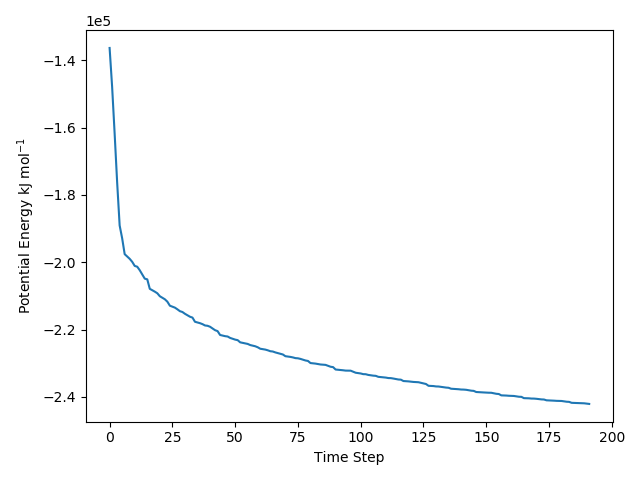
\includegraphics[scale=0.4]{HairE}
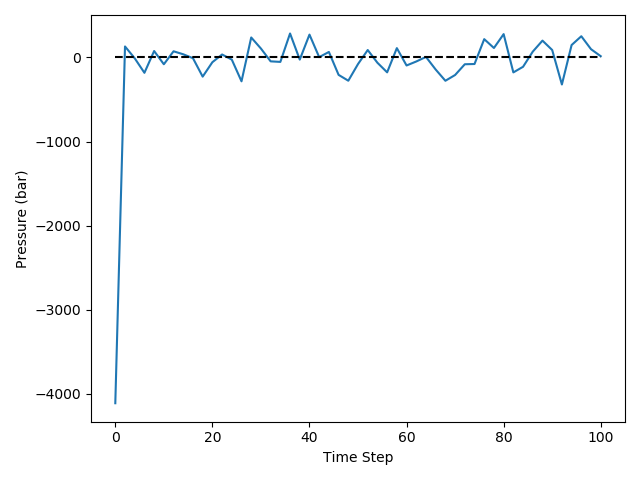
\includegraphics[scale=0.4]{HairNPTP}
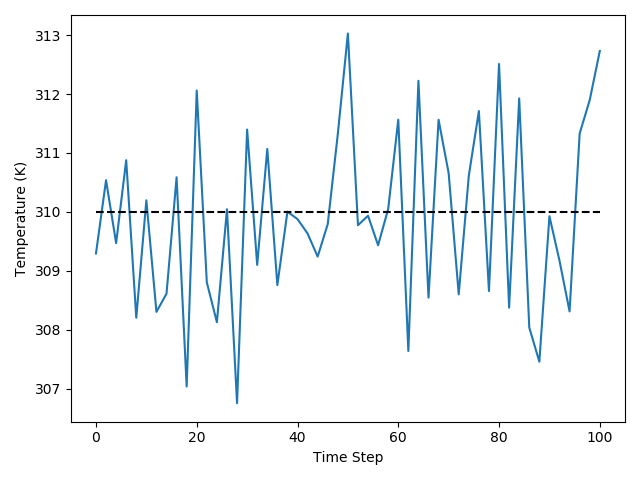
\includegraphics[scale=0.4]{HairNPTT}
\caption{Various properties of the hairpin stucture during energy minimisation and thermal equilibration.  Top left - the potential energy during the minimisation, top right - the pressure during the equilibration, bottom - the temperature during equilibration.  The black lines shown are the reference pressure and temperature 1.0 bar and 310K.}
\end{figure}

\subsection{Simulations}

In this subsection we outline the aspects of the molecular dynamics simulations that were performed both as part of the pulling simulations and the umbrella sampling simulations.

\subsubsection{Pulling}

Simulating the pulling of the proteins is an example of a steered molecular dynamics simulation\cite{GMX}.  In pulling one group within the protein with respect to another, work must be applied to the system and therefore the system is no longer in equilibrium\cite{GMX}.  One can infer the free-energy difference between different pulling distances through the Jarzynski relation \cite{Jar} which relates the average work done on a system (a non-equilibrium property) to the free energy difference (an equilibrium property).\\

The exact nature of the pulling can be performed in a number of ways.  One possibility is to apply a constant force to the center of mass of the two groups in which one is interested\cite{GMX}.  In the pulling simulations that we will analyse, a different option was taken which is to apply a harmonic potential to the centres of mass of the group one wishes to pull\cite{GMX}.  One can visualise this as attaching a spring with a certain force constant to the centre of mass, the other end of the spring is then pulled away from the reference group at some constant rate which the user has defined.  In such a pulling simulation the force applied (and the work done) is not constant but rather will be dependent upon the interactions between the different groups in the molecule\cite{GMX}.\\

Pulling simulations were performed on both of the structures which we have described.  In the case of the helix structure we will show results directly from the pulling simulations in the results section.  For the hairpin the pulling simulation offered a start point for the umbrella sampling, the results of which will be shown later.  Here we will describe the nature of the steered molecular dynamical simulations performed on the two systems.\\

For the helix structure a leap-frog algorithm \cite{GMX} was used for integration of the equations of motion with a time step of 0.002ps.  Temperature was coupled separately for the protein and non-protein groups using a Nos\' e-Hoover \cite{NH} extended ensemble with Parrinello-Rahman \cite{PR} pressure coupling.  Boundaries were periodic in all directions.  As we have described, harmonic umbrella pulling was carried out using a harmonic spring constant of 1000 kJ mol$^{-1}$ nm$^{-2}$.  The pulled group comprised atoms 136-155 (residue SER) with the first residue (LEU atoms 1-11) used as the reference.  Four different pulling rates were used 0.1, 0.01, 0.001 and 0.0001 nm ps$^{-1}$.\\  

The hairpin pulling simulation was carried out in exactly the same manner.  With the C-terminal being pulled at a rate of 0.01 nm ps$^{-1}$ from the reference group which was the N-terminal.


\subsubsection{Umbrella Sampling}

The configurations of the structures obtained in non-equilibrium pulling simulations can be used as the start points for umbrella sampling simulations.  Starting from the structures generated in the pulling simulations one can then perform thermal equilibration in the normal manner but with the additional bias potential required for the umbrella sampling method\cite{GMX}.\\

For each window both the thermal equilibration and molecular dynamics simulations were performed in exactly the same way as for the pulling simulations but with the pulling rate set to zero and the harmonic force constant reduced to 500 kJ mol$^{-1}$ nm$^{-2}$. 

\section{Results and Discussion}

We now show the results obtained from the various simulations that were performed, starting with the results of the pulling simulations on the helix.  

\subsection{Pulling Simulations}

In this section we present the results and analyses of pulling simulations performed on the helix structure.  Four different simulations were run in each of which the helix was pulled at a different speed, namely 0.1, 0.01, 0.001, 0.0001 nm ps$^{-1}$.  Below (figure 4) we show the visualisations of the state of the molecule at three time steps along the course of the four trajectories.  All visualisations were created using VMD \cite{VMD}.  The initial configuration was the state obtained by energy minimisation and equilibration that we explained in section 3.\\

\begin{figure}[h!]
a)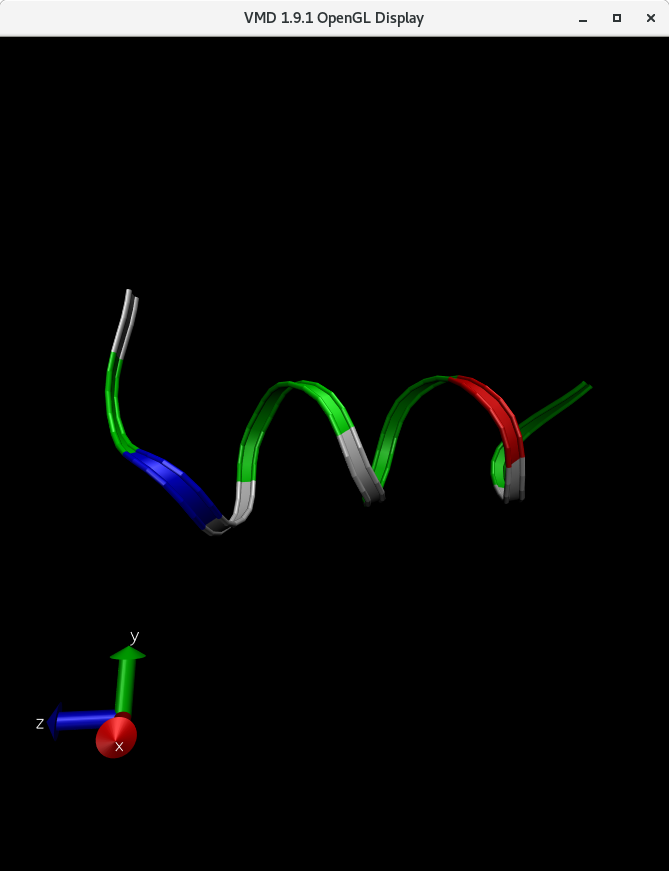
\includegraphics[scale=0.2]{First01}\\

b) 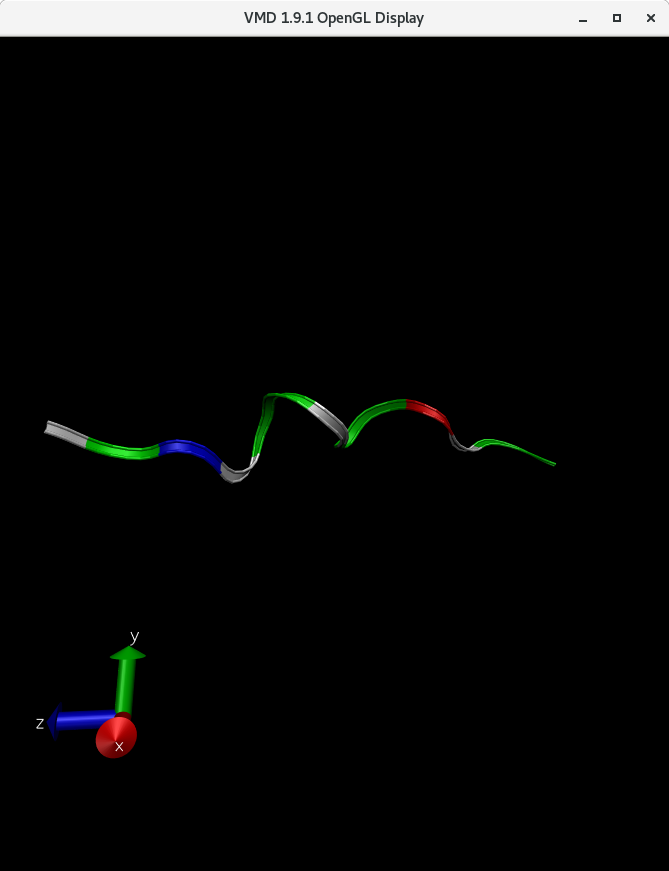
\includegraphics[scale=0.15]{301}
c)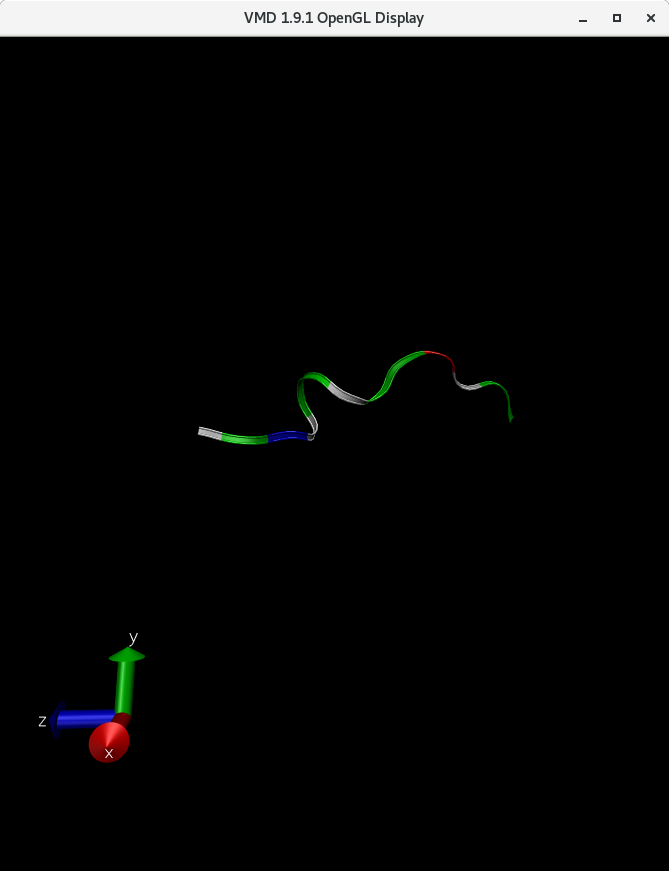
\includegraphics[scale=0.15]{16_001}
d)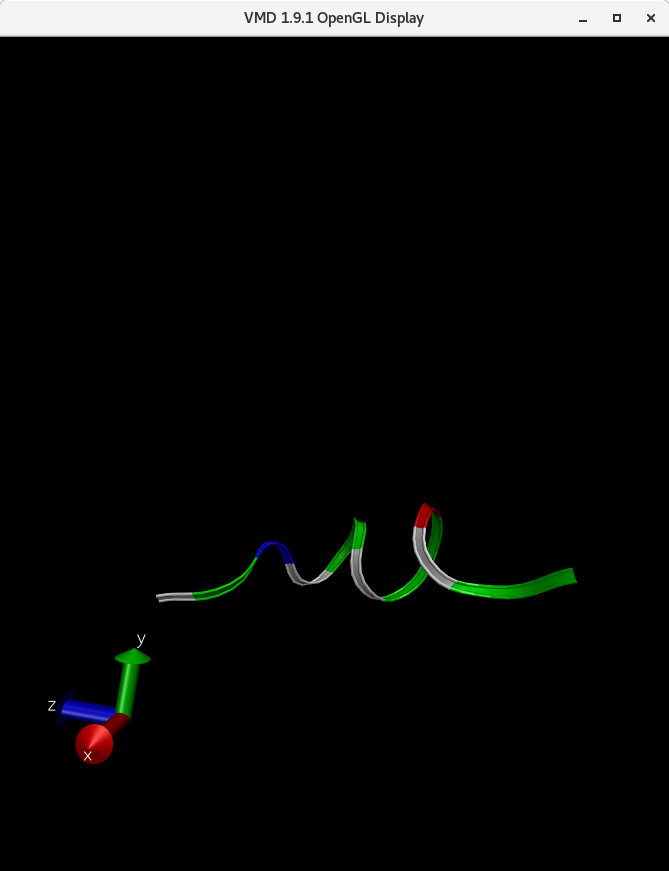
\includegraphics[scale=0.15]{50_0001}
e) 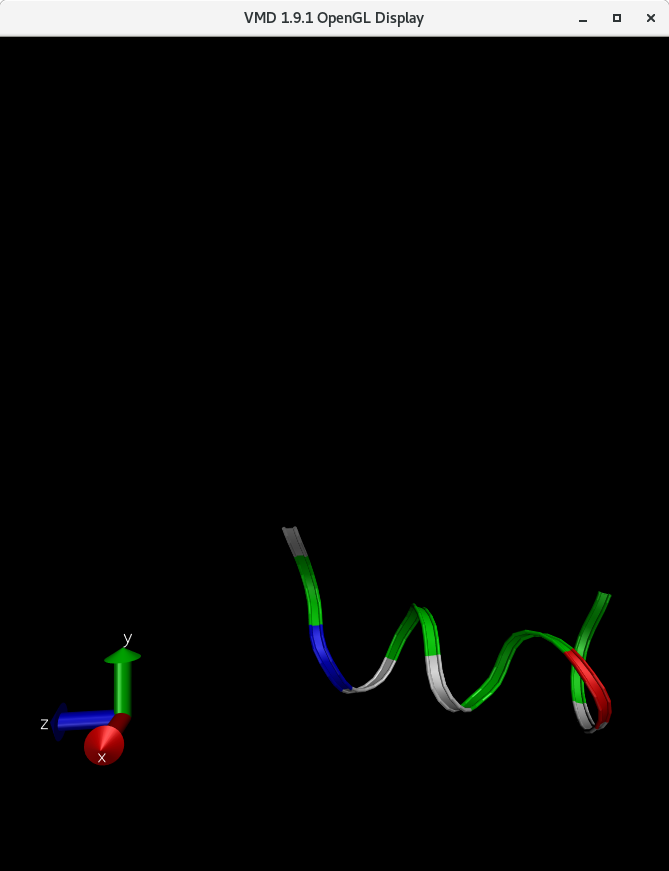
\includegraphics[scale=0.15]{50_00001}\\

f)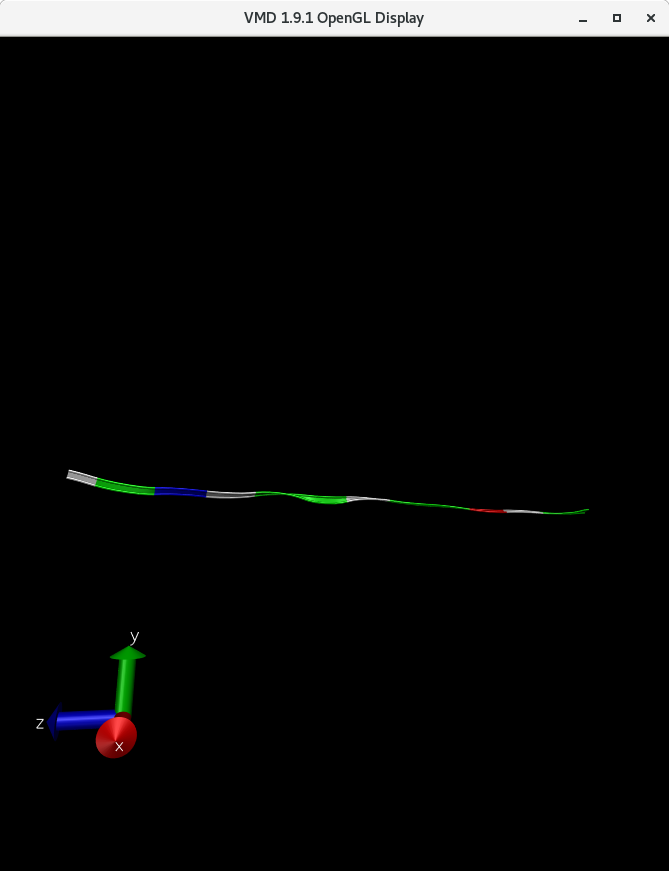
\includegraphics[scale=0.15]{Last01}
g)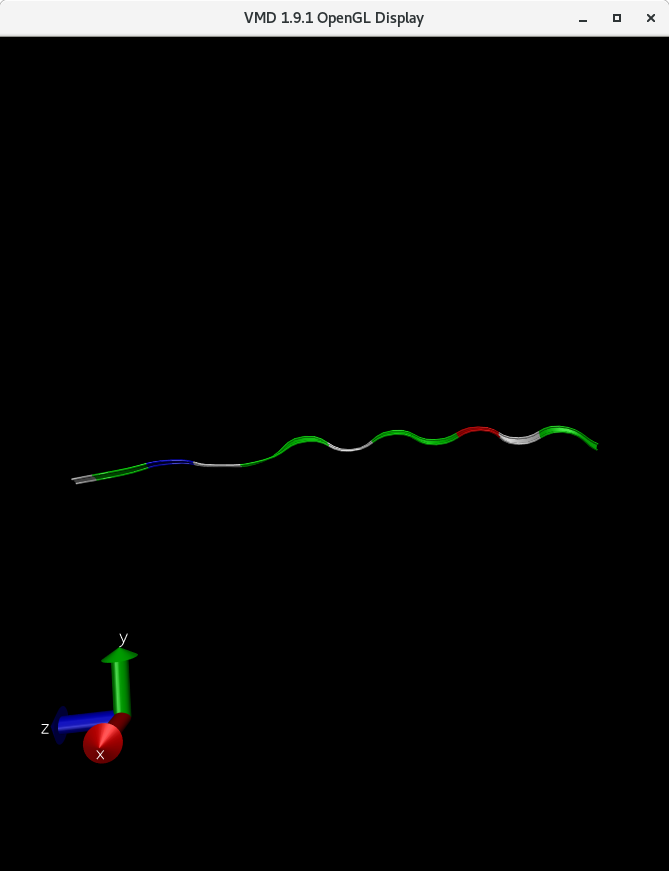
\includegraphics[scale=0.15]{40_001}
h)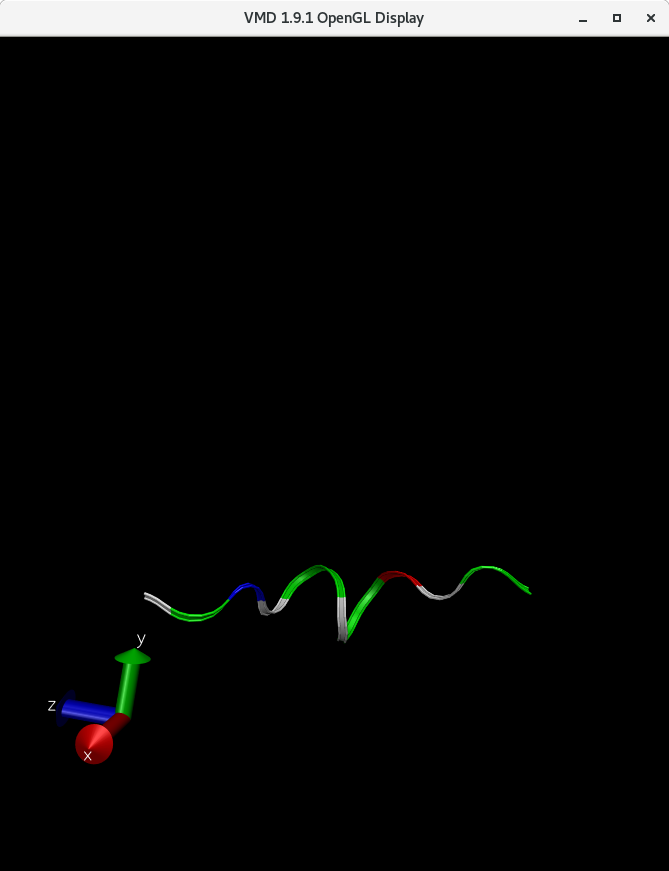
\includegraphics[scale=0.15]{Last0001}
i)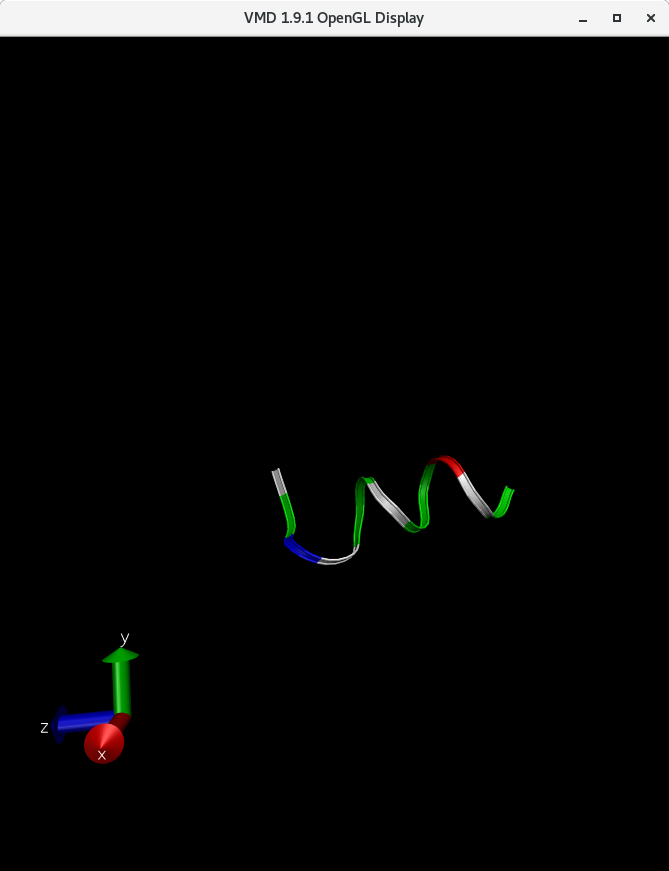
\includegraphics[scale=0.15]{Last00001}
\caption{Visualisation of the helix at different stages during the four simulations.  Across the two rows below, we have snapshots taken from (left to right) the 0.1, 0.01, 0.001 and 0.0001 nm/ps simulations.  The first row (b-e) shows respectively the 3rd, 16th, 50th and 50th time-steps of the relevant simulation while the final row (f-i) shows the helix at the last time-step}
\end{figure}

Over the course of the simulations the force required to maintain the pulling speed was recorded as well as the end to end distance.  We show plots of force vs. distance for the four simulations in figure 5.\\

\begin{figure}[h!]
\label{fig: FDs}
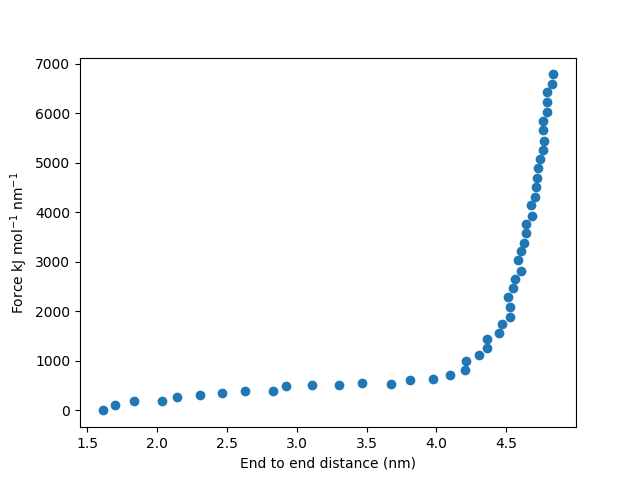
\includegraphics[scale=0.4]{FD0_1}
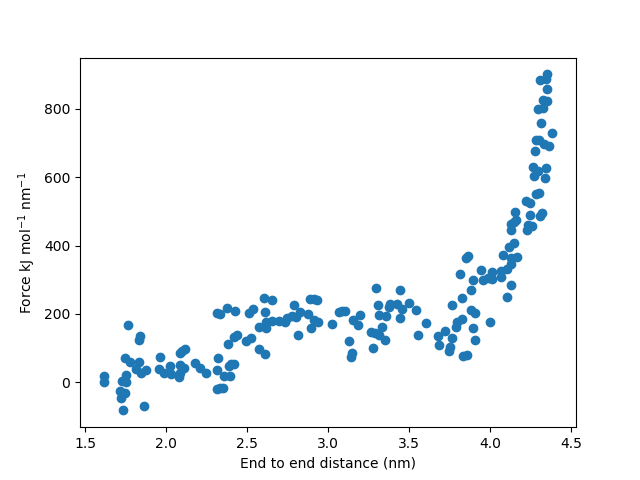
\includegraphics[scale=0.4]{FD0_01}
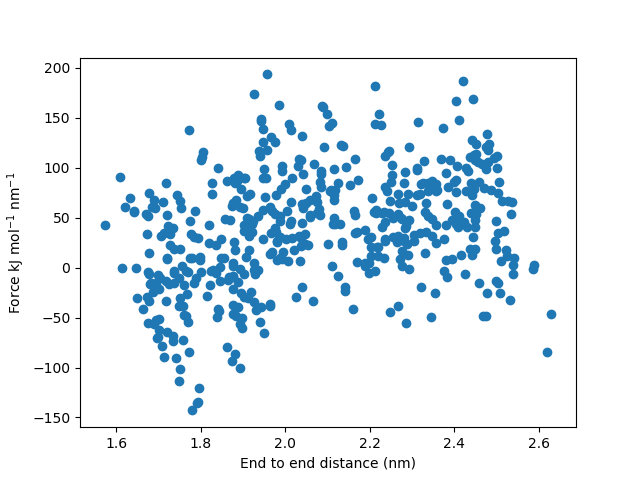
\includegraphics[scale=0.4]{FD0_001}
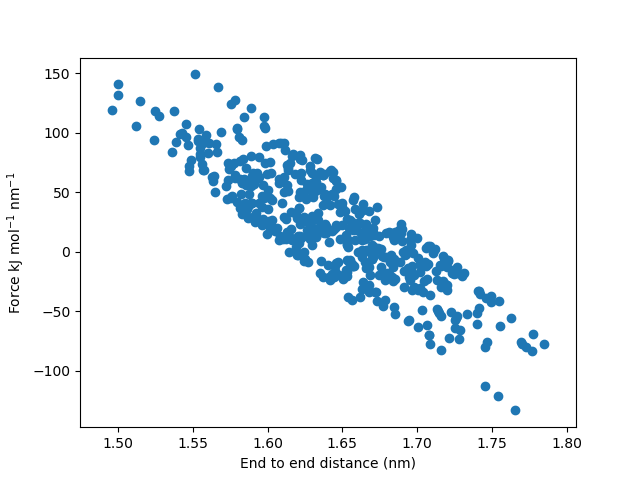
\includegraphics[scale=0.4]{FD0_0001}
\caption{Force required to maintain pulling speed as a function to end to end distance for the four trajectories.  Top - left 0.1 nm ps$^{-1}$ , right 0.01 nm ps$^{-1}$; Bottom - left 0.001 nm ps$^{-1}$, right 0.0001 nm ps$^{-1}$.}
\end{figure}

For the two faster pulling simulations (0.1, 0.01 nm ps$^{-1}$) the force shows a clear trend of increasing slowly with distance up to around 4nm and then increasing much more rapidly.  The sharp increase in force required for larger end to end distance represent the fact that at such scales the protein is being ripped apart.  The slower the pulling was performed, however, the stronger the noise and so in the slower pulling simulations the noise completely dominates.  In fact for the 0.001 and 0.0001 nm ps$^{-1}$ simulations the distributions can be well approximated as multivariate Gaussians with mean and covariance estimated from the data, as shown in figure 6.\\ 
 
\begin{figure}[h!]
\label{fig: FDGs}
a)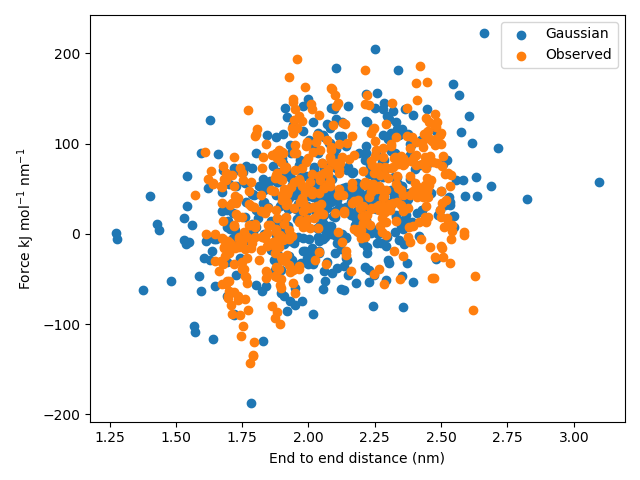
\includegraphics[scale=0.4]{FDG1}
b)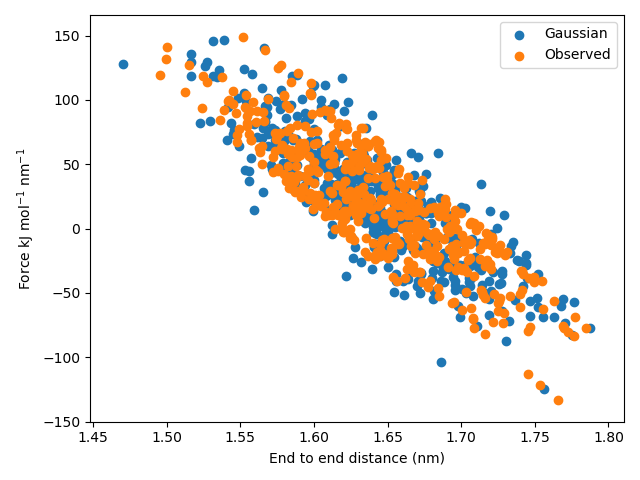
\includegraphics[scale=0.4]{FDG2}
\caption{In orange the observed force against end to end distance for the 0.001 nm ps$^{-1}$ (left) and 0.0001nm ps$^{-1}$ (right) pulling trajectories.  The blue points represent bivariate Gaussians with mean and covariance calculated from the observed data.}
\end{figure}

It appears therefore that a stochastic Gaussian noise dominates when the pulling velocity is small.  It is also notable that for the slowest of the simulations, the force and distance are highly correlated with correlation coefficient $r = -0.85$ compared to $r = 0.33$ for the 0.001 nm ps$^{-1}$ simulation.\\


Over the course of the pulling simulation the radius of gyration and the end-to-end C-$\alpha$ distance were also recorded.  For a given system the radius of gyration $R_g$ is the distance from an axis at which a point mass, with mass equal to that of the system, would have the same moment of inertia as the entire system.  It is a useful description of the conformation of a protein \cite{Rgyr} and is given by the following formula

\begin{equation}
R_g^2 = \frac{1}{M}\sum_i m_i (\vec{r}_i \vec{R}_c )^2, 
\end{equation}

where $m_i$ is the mass of the atom located at position $\vec{r}_i$, $\vec{R}_c$ is the location of the centre of mass and $M$ is the combined mass of the atoms.  For a system in which all the masses are equal $R_g^2$ is simply the mean square displacement from the centre of mass.  In the case of inhomogeneous masses it is the weighted average displacement.  We show in figure 7 the radius of gyration and end-to-end distances over the course of the four trajectories.\\

\begin{figure}[h!]
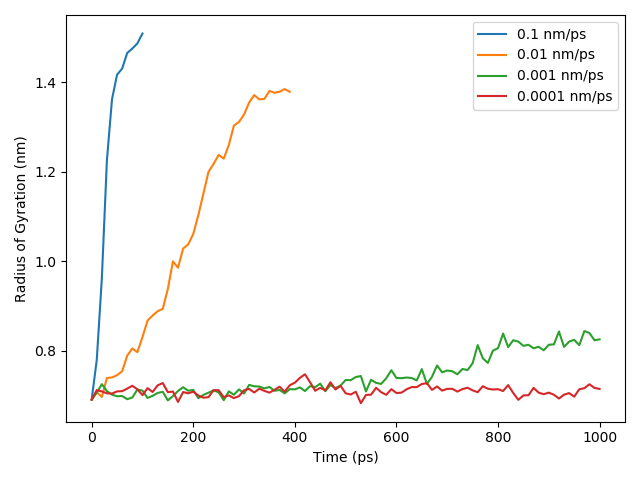
\includegraphics[scale=0.4]{RGYR}
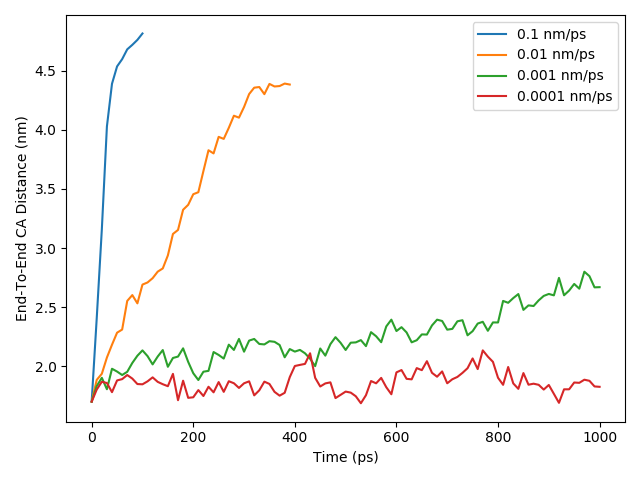
\includegraphics[scale=0.4]{E2E}
\caption{The radius of gyration (left) and end to end C-$\alpha$ distances  (right) over the entire course of each of the four trajectories (shown in different colours).}
\end{figure}

As we can see the two plots follow a similar trend.  For the faster velocities the pulling dominates and both the radius of gyration and end-to-end distance increase before plateauing towards the end of the simulation (as the protein begins to be ripped apart).  For the slower pulling rates the intermolecular forces dominate and the end-to-end distance and radius of gyration become dominated by noise.  This is exactly the same behaviour as we saw for the force-distance plots.\\

One link between the radius of gyration and the end-to-end distance can be seen in the case of an ideal chain\cite{IdCh}.  An ideal chain is a simple model of a polymer comprising $n$ non-interacting monomers of equal length.  In this simplistic model the end-to-end distance should be normally distributed and the radius of gyration related to the end-to-end distance by $\langle R^2_g \rangle = \langle R^2 \rangle / 6$ (where $R$ is the end-to-end distance)\cite{IdCh}.  We show histograms of the end-to-end distance for the four trajectories.  We also show for reference Gaussians with the same mean and variance as the data.\\

\begin{figure}
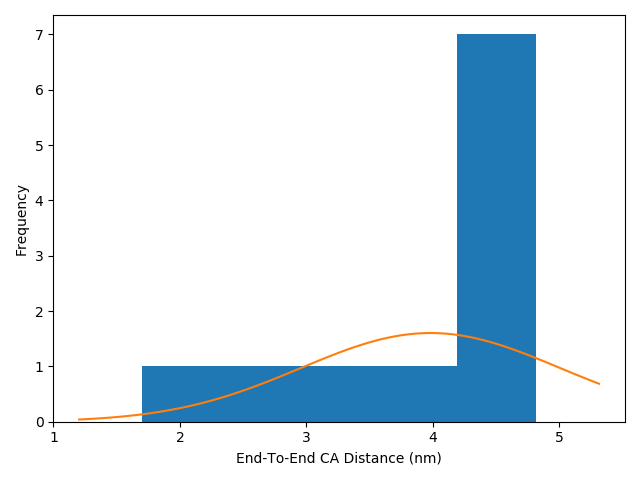
\includegraphics[scale=0.33]{E2EH1}
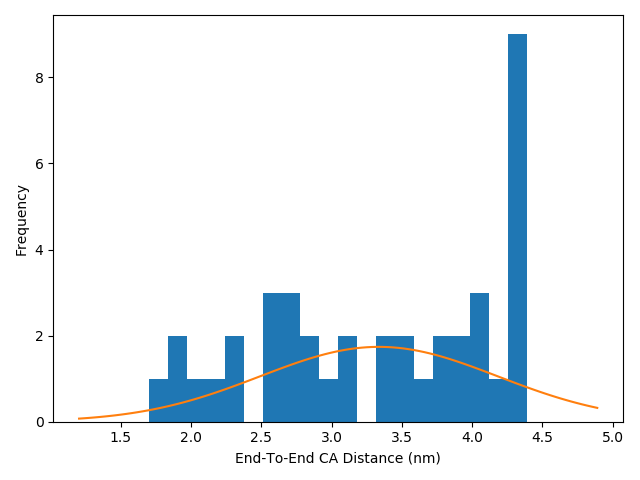
\includegraphics[scale=0.33]{E2EH2}
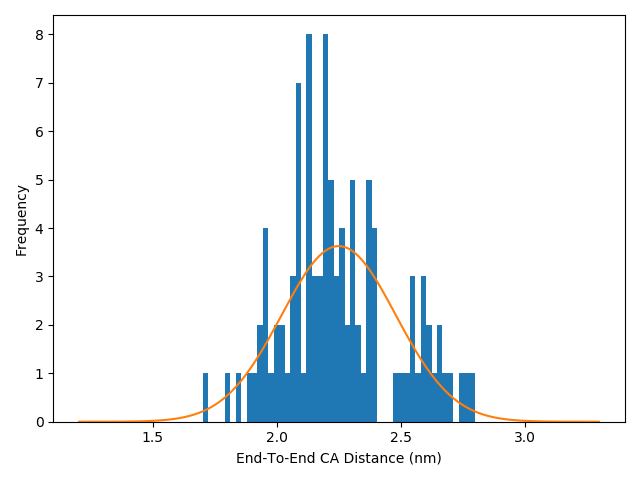
\includegraphics[scale=0.33]{E2EH3}
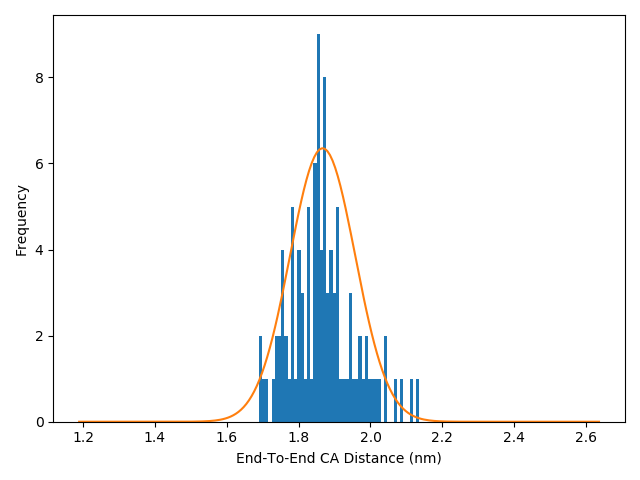
\includegraphics[scale=0.33]{E2EH4}
\caption{Histograms of the end to end distance over the course of the four different trajectories (top left 0.1 nm ps$^{-1}$; top right 0.01 nm ps$^{-1}$; bottom left 0.001 nm ps$^{-1}$; bottom right 0.0001 nm ps$^{-1}$.  For each plot a Gaussian, with mean and variance calculated from the data, is shown for reference.  The means in decreasing order of pulling speed were
4.0 $\pm$ 1 nm, 3.3 $\pm$ 0.8 nm, 2.3 $\pm$ 0.2 nm and 1.9$\pm$0.1 nm where the uncertainty shown is the standard deviation.}
\end{figure}

For the fastest simulations the frequency of end-to-end distances is more or less constant as the protein is pulled until it begins to plateau at the end of the simulation, represented by a large spike in frequency for the largest distances.  Clearly a Gaussian is not a good fit for the faster pulling speeds and therefore an ideal chain is a poor approximation of the protein.  On the other hand, for the slower pulling trajectories the Gaussian approximation qualitatively appears a good fit.  Taking the ratio of the average end-to-end distance and mean radius of gyration one finds values of 3.0 for the 0.001 nm ps$^{-1}$ simulation and 2.6 for the 0.0001 nm ps$^{-1}$ trajectory.  Therefore the ideal chain is still a poor approximation of the molecule.  

\subsection{Umbrella Sampling Simulations}  

In this subsection we show the results of the Umbrella Sampling simulations that were carried out for both the $\alpha$-helix and $\beta$-hairpin structures.  For each structure we will show the derived PMFs \cite{GWHAM} along a given reaction coordinate, we will also show the uncertainty on these values derived from Bayesian bootstrapping\cite{GWHAM}.  Finally we will explore the overlap of the umbrella histograms and discuss the impact of this on the other results. 

\subsubsection{$\alpha$ - helix}

For the $\alpha$-helix the system was aligned along the $z$-axis, the reaction coordinate was the end-to-end distance along the $z$-axis and 25 umbrella windows with harmonic biases were simulated.  The PMF was calculated from the histograms produced using WHAM as described in section 2.  Bayesian bootstrapping was also carried out to estimate the uncertainty in the results.  The number of iterations of the bootstrap was found to affect the estimated uncertainty.  To quantify this the average (over all values of reaction coordinate $z$) of the standard deviation of the PMF was calculated for several different numbers of iterations the results are shown in figure 9.  The general trend appears to be an increase in average standard deviation until the number of iterations was around 100 we therefore chose to use the standard deviations calculated from 100 bootstraps as our uncertainties in the PMF.\\ 

\begin{figure}[h!]
\label{fig: helboot}
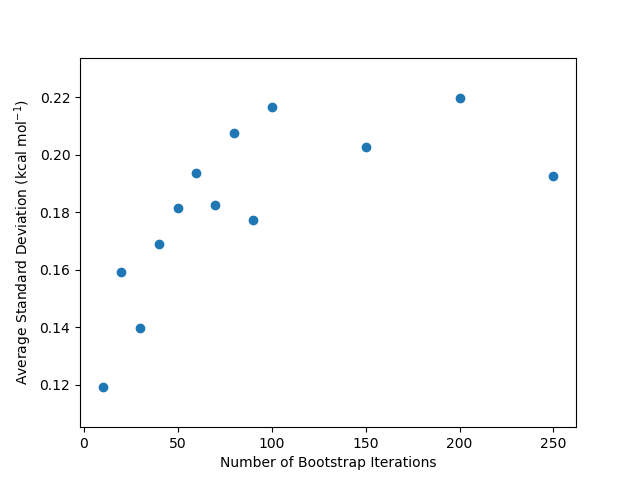
\includegraphics[scale=0.5]{HelBootstrapSDev}
\caption{The effect of increasing the number of bootstrap iterations on the average (over $z$-axis) standard deviation of the calculated PMF}
\end{figure}

The PMF calculated using WHAM on the umbrella histograms is shown in figure 10 alongside the calculated results $\pm 3 \sigma$ and $\pm 5 \sigma$.\\ 

\begin{figure}[h!]
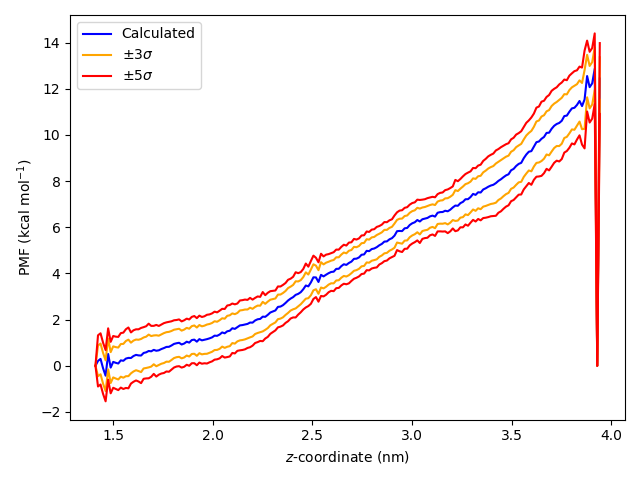
\includegraphics[scale=0.5]{helPMF}
\label{fig: helPMF}
\caption{PMF calculated from umbrella histograms using WHAM is shown in blue.  The orange and red curves are the calculated PMF $\pm 3 \sigma$ and $\pm 5 \sigma$ respectively and are shown for reference.}
\end{figure}

 As the distance along the $z$-axis increases so too does the PMF as expected due to the equilibrium system being that at the lowest $z$ value.  There are however some large spikes in the data most notably between around 3.9 nm but also  at around 1.4 nm and less so at approximately 2.5 nm.\\
 
To quantify the spikes we looked at the absolute difference between the PMF calculated at a given value of $z$ and that calculated at the previous value of reaction coordinate.  We then took the mean of these absolute differences and any values of $z$ for which the absolute difference exceeded the mean were considered a spike.  We plot the absolute values of the differences and also show a histogram of spike locations in figure 11.\\


\begin{figure}[h!]
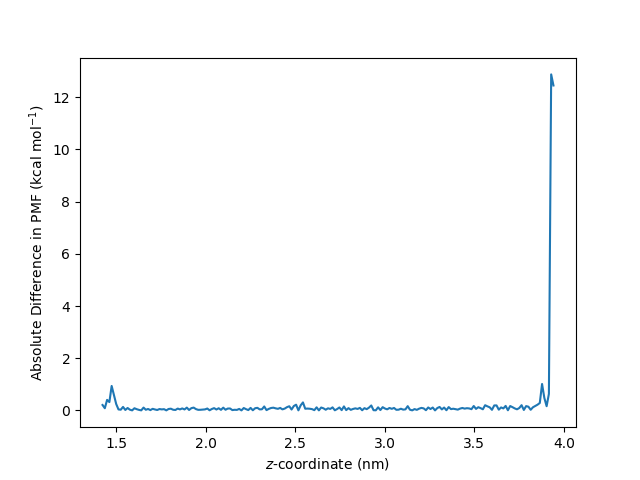
\includegraphics[scale=0.4]{HelAbsDiffs}
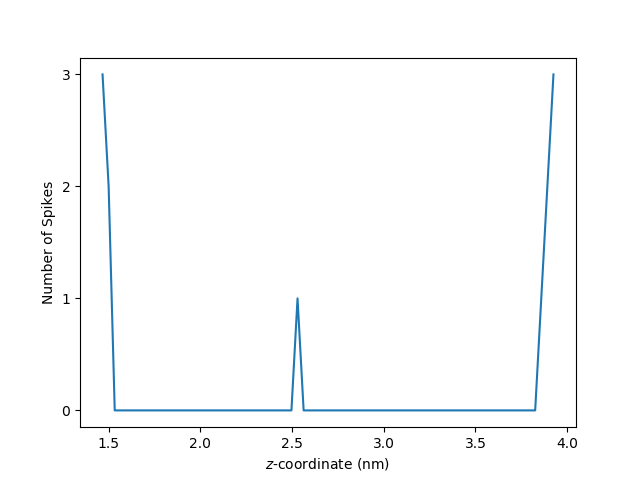
\includegraphics[scale=0.4]{HelSpikeHist}
\label{fig: helSpikes}
\caption{Left - the absolute difference between consecutive values of the PMF.  Right - the frequency of values greater than the mean of the absolute difference in consecutive PMF values.}
\end{figure}
 
As we described in section 2 it is important that every value of the reaction coordinate is well sampled \cite{Umbrella}, this is ensured by having sufficient overlap \cite{GWHAM} in the umbrella histograms such that the reaction coordinates far from energy minima are still sampled.\\

We hypothesised that the cause of the spikes in the PMF was insufficient sampling in certain regions of the reaction coordinate.  To test this hypothesis we employed a number of techniques starting with simply inspecting the histograms, these are shown in figure 12.\\

\begin{figure}[h!]
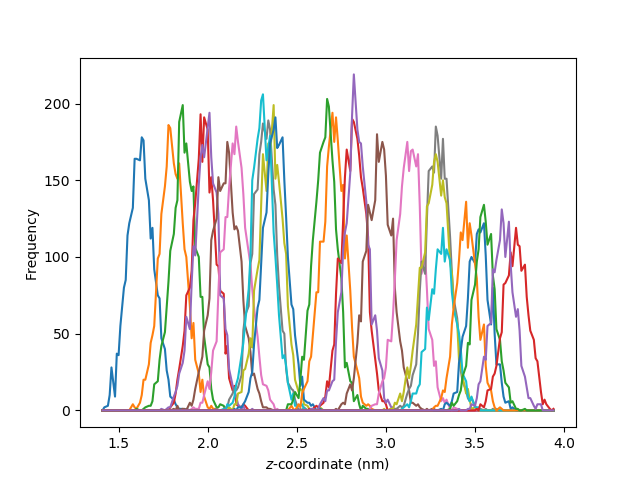
\includegraphics[scale=0.5]{HelUMBs}
\label{fig: HelUmbHists}
\caption{The 25 histograms corresponding to the different umbrella windows used to sample the entire range of $z$ for the helix.}
\end{figure}

By inspection we can see that there is little sampling at the two extremes of the reaction coordinate and also there appears to be a gap centred at $z \approx 2.5$nm, all of which coincide with the spikes seen in the PMF.  To better visualise this we took the sum of all histograms at each value of $z$, this is shown in figure 13.\\

\begin{figure}[h!]
\includegraphics[scale=0.5]{HelUMBSums}
\label{fig: HelUmbSum}
\caption{The total number of times at which the system occupied a given value of $z$ across all the umbrella sampling windows.}
\end{figure}

Here we can more clearly see that there is very little sampling at either extreme of $z$ and also another minimum close to 2.5nm. More precisely there were fewer than 100 samples at each point (i.e. in each bin centred around) in the ranges 1.41-1.54nm, 2.49-2.56nm and 3.79-3.94nm.  In fact there are 10 points at which there are fewer than 10 samples and 2 which were not visited at all.  The smallest value close to 2.5nm occurred in the bin centred at 2.52nm which was only visited 56 times across all simulations.  This result appears to agree with the hypothesis that the lack of sampling in the simulations was the cause of the spikes in the PMF.  Note that there was also a minimum around 3.0nm, which can also be seen in figure 12 as at that location only two histograms appear to overlap.  However in this region the minimum sampling was 171 occurrences (bin centred at 3.05nm) and there is no significant spike in the PMF.\\

We also decided to look more closely at the overlap between the histograms, this we did in two ways.  Firstly, we characterize the overlap by the value of the second largest frequency at each given point.  This is related to the overlap since a value of zero implies that at most one histogram contributed to sampling at that point, while any non-zero value indicates that at least two histograms overlapped in that region.  The larger the value of the second maximum the greater the overlap.  We show the results of the second maxima in figure 14.\\  

\begin{figure}[h!]
\includegraphics[scale=0.5]{HelUMBScnd}
\label{fig: HelUmbScnd}
\caption{The second largest number of visits to each point along the $z$-axis.  A value of zero indicates that at most one window sampled that location.}
\end{figure}

Once more we see that the smallest values occur in the regions where spikes were located in the PMF.  In this case the minimum occuring around 2.5nm (12 visits at 2.51nm) was much closer to the minimum occuring around 3.0nm (21 samples at 2.99nm and 3.13 nm) but the predominant minima were still those in which spikes were located.\\

The second way in which we quantified overlap was to look at the area shared between each pair of histograms.  We define the overlap $I_{ij}$ of histogram $h_i$ and histogram $h_j$ as \cite{Over}

\begin{equation}
I_{ij} = \frac{\sum_{k = 1}^{N_b} \min(h_i^{(k)},  h_j^{(k)})}{\sum_{k = 1}^{N_b} h_i^{(k)}},
\end{equation}

where $N_b$ is the number of bins in the two histograms and $h_i^{(k)}$ is the frequency in bin $k$ of histogram $h_i$.  Note that the bins (not just the number) used must be the same for both histograms.  The denominator is a normalising factor such that $I_{ij} \in [0, 1]$ with unity if and only if the values are the same in both histograms in every bin.  In general the overlap is asymmetric $I_{ij} \neq I_{ji}$ however if the same number of samples appear in both histograms then it will be symmetric.  In our cases there were different number of samples in the different windows and therefore the overlap was asymmetric.\\

For our data we arranged the histograms such that the positions of the maxima of the histograms were in increasing order.  We then calculated the overlap between each pair of histograms (in each direction)  (i.e. $I_{ij}$ and $I_{ji}$) and show these values in figure 15.\\

\begin{figure}[h!]
\includegraphics[scale=0.5]{HelUMBOverOrd}
\label{fig: HelUmbOver}
\caption{Heatmap showing the overlap matrix with elements $I_{yx}$.}  
\end{figure}

The terms on the diagonal are one since the overlap of a histogram with itself is trivially unity.  We can see that in some regions many histograms overlap with each other, this is represented by non-zero overlaps several spaces from the diagonal, whereas in other areas there is little to no overlap with histograms other than the nearest neighbours.  The most obvious lack of overlap occurs between histograms 11 and 12 for which the overlap was only 0.04 which is barely visible on the plot.  The maxima of these two histograms were at 2.38nm and 2.70nm respectively and so the lack of overlap between these nearest neighbours is another indicator that the region close to 2.5nm was poorly sampled leading to the spike in the PMF.     

\subsubsection{$\beta$-hairpin}

In the case of the $\beta$-hairpin once more the $z$-axis was used as the reaction coordinate.  In order for this to be a sensible reaction coordinate to distinguish between the folded hairpin state and the unfolded state, the molecule was therefore aligned such that the two ends of the hairpin were always oriented along the $z$-axis.  Unfolding was therefore represented by increasing $z$.  For this molecule there were 21 structures and we show visualisations of the protein in windows 1, 10 and 21 in figure 16.  One can clearly see that the molecule is deformed from a folded hairpin to a straight line.\\

\begin{figure}[h!]
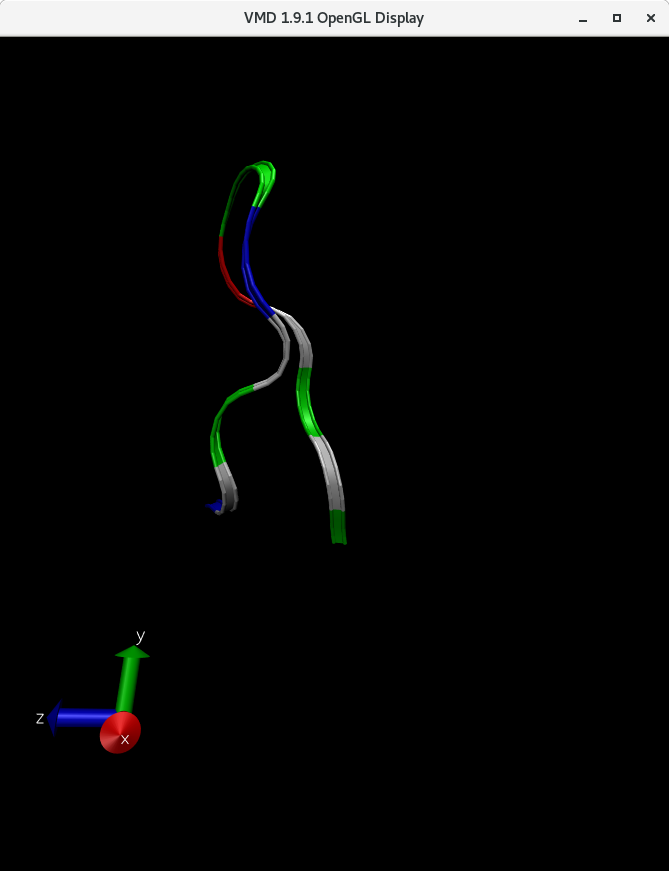
\includegraphics[scale=0.2]{HairpinFirstRibbons}
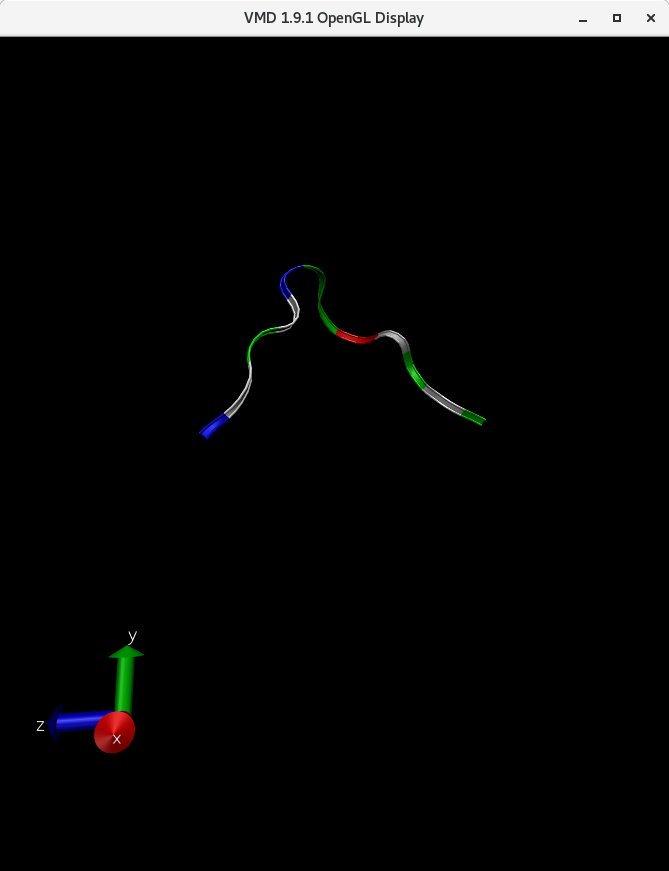
\includegraphics[scale=0.2]{Hairpin10Ribbons}
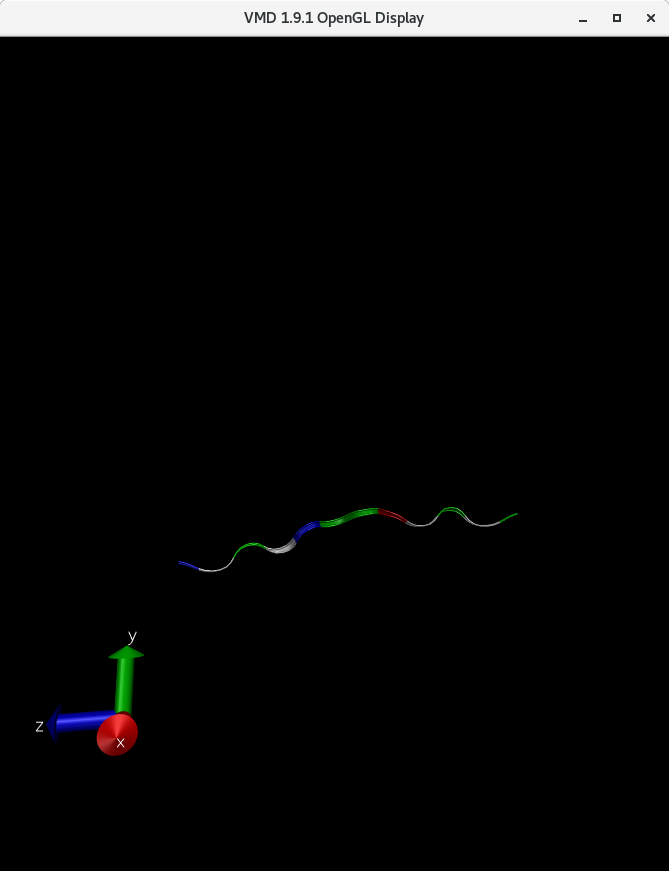
\includegraphics[scale=0.2]{HairpinLastRibbons}
\label{fig: HairpinVis}
\caption{The initial state of the hairpin in the 1st, 10th and 21th windows of the umbrella sampling simulation.}
\end{figure}

As for the helix, the PMF was calculated from the umbrella simulations using WHAM and the uncertainty was calculated using Bayesian bootstrapping.  We show (figure 17) the effect of number of bootstrap iterations on the average standard deviation below. \\

\begin{figure}[h!]
\label{fig: hairboot}
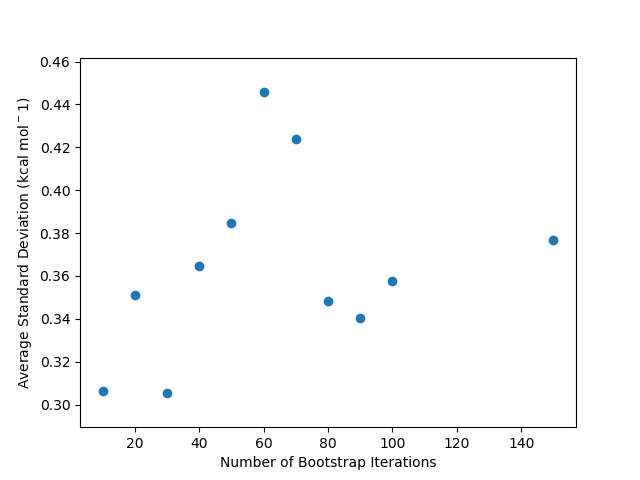
\includegraphics[scale=0.5]{HairBootstrapSDev}
\caption{The effect of increasing the number of bootstrap iterations on the average standard deviation of the PMF.}
\end{figure}

Unlike for the helix there is no clear trend.  We elected to use the 150 bootstrap iterations standard deviation $\sigma$ as an estimate for the uncertainty.  Once more we show the calculated PMF together with $\pm 3\sigma, \pm 5 \sigma$ boundaries in figure 18. \\

\begin{figure}[h!]
\label{fig: hairpmf}
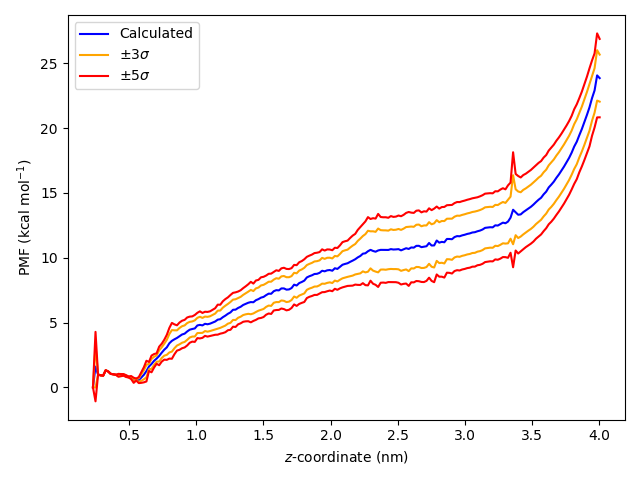
\includegraphics[scale=0.5]{hairPMF}
\caption{PMF calculated (blue), using WHAM, from histograms obtained in umbrella sampling simulations of the hairpin.  The orange and red curves represent  the calculated PMF $\pm 3\sigma$ and $\pm 5 \sigma$ where $\sigma$ is the standard deviation calculated from bootstrappping.}
\end{figure}

The shape is appears rather different compared to the helix.  Here we appear to have a period of fairly constant PMF until $z \approx 0.7$nm at which point we have a similar shape to that for the helix until $z \approx 2.2$nm when the rate of increase in PMF grows with $z$.  Again, however, we have the presence of spikes in the PMF curve which we hypothesis to be the result of a lack of sampling in those regions.  From the plot the main spikes appear to be around 0.25nm and 3.3nm.\\

The changing shape of the curve means that we cannot simply take the absolute differences as before since spikes will appear in the final section where the gradient is increasing dramatically.  We therefore chose to approximate the curve by a linear region up to $z = 2.24$ followed by a quadratic region.  In the linear region we took the absolute difference between consecutive value and calculated the mean $\mu_1$ and standard deviation $\sigma_1$, any points for which the absolute difference exceeded $c_1 = \mu_1 + \sigma_1$ were taken to be spikes.  In the quadratic region the same process was performed but for the absolute value of the second difference between consecutive points.  Again the mean $\mu_2$ and standard deviation $\sigma_2$ were calculated and any points above the cut-off $c_2 = \mu_2 + \sigma_2$ were taken to be a spike.  The choice to increase the cut-off by a standard deviation compared to the cut-off we used for the helix was motivated by the lack of an extremely large difference as we had for the helix.  The first and second differences used and a histogram of the positions of the spikes are shown in figure 19.\\ 

\begin{figure}[h!]
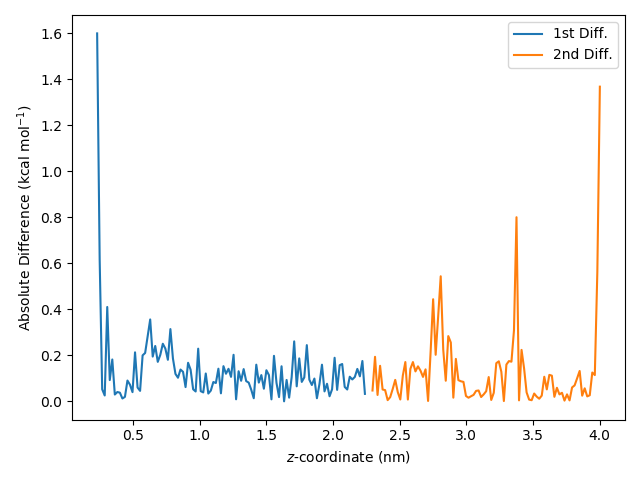
\includegraphics[scale=0.4]{HairAbs}
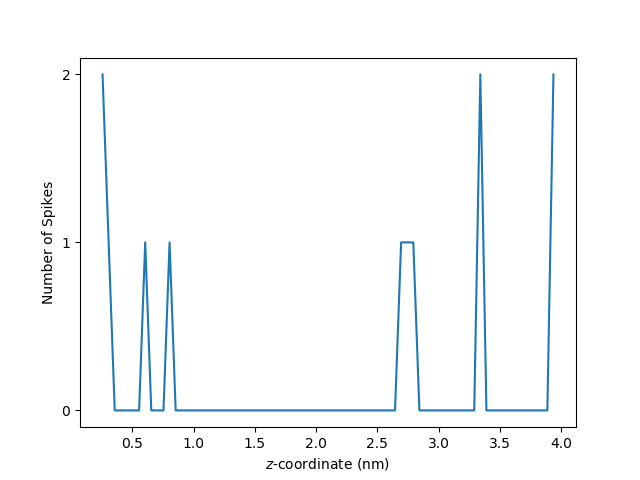
\includegraphics[scale=0.44]{HairSpikes}
\label{fig: hairSpikes}
\caption{Left - up to $z = 2.24$ nm the absolute value (blue) in difference between consecutive values of PMF followed by the absolute value in second difference (orange).  The frequency of spikes as a function of $z$.}
\end{figure}

The spikes around 0.25, 3.3 and 3.9nm are obvious from the PMF plot while the others we have found are less clear in the original plot.  We then performed the same analyses as for the helix to determine if the spikes could be explained by undersampling of certain regions.  We first show (figure 20) the raw histograms and the total frequency across all histograms.\\

\begin{figure}[h!]
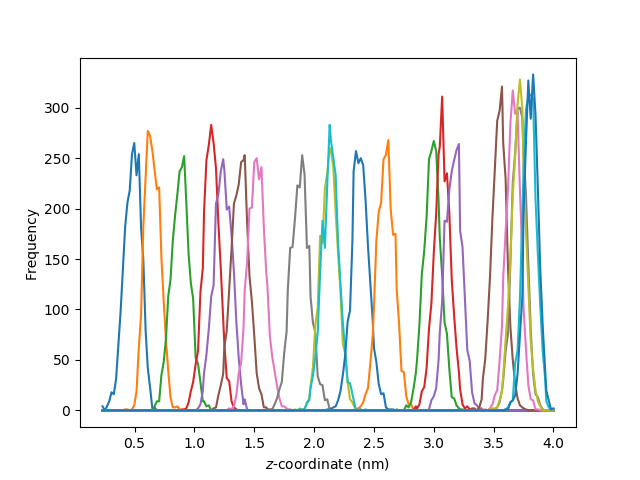
\includegraphics[scale=0.4]{HairUMBs}
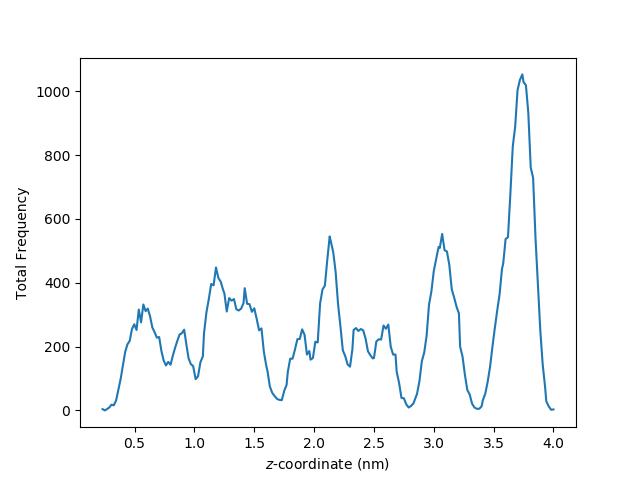
\includegraphics[scale=0.4]{HairUmbSums}
\label{fig: hairhists}
\caption{Umbrella histograms for the different windows of simulation of the hairpin (left) with the total frequencies at each $z$ across all windows (right).}
\end{figure}

For the raw histograms we can see that there appears to be gaps in the sampling occurring at around 0.2, 2.8, 3.3 and 4nm all of which have corresponding spikes in the PMF.  The spikes at 0.6 and 0.8 nm have corresponding gaps in the histograms as well, although far smaller than the others.  There is also an apparent undersampling at around 1.7nm which is not borne out as a large spike in the PMF although there is a subtle change visible in that vicinity in the PMF.\\

Finally we show (figure 21) the second maximum frequency and overlap heat map both of which tell us how much the histograms are overlapping with each other.\\   

\begin{figure}[h!]
\includegraphics[scale=0.4]{HairUMBScnd}
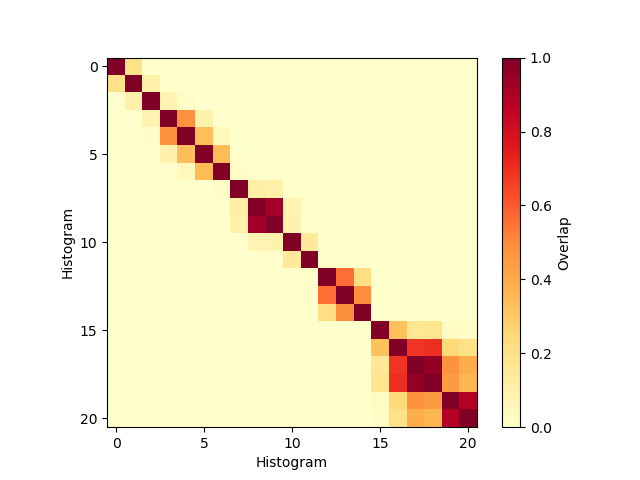
\includegraphics[scale=0.4]{HairUmbOverOrd}
\label{fig: hairover}
\caption{Left - the second highest number of visits to each value of $z$ across all windows.  Right - a heatmap of the overlap $I_{yx}$.}
\end{figure}

In the second maxima plot we can see that the regions in which we detected spikes also have a very low second maximum frequency indicating low overlap.  Likewise in the heatmap we can see that in some places there is very limited overlap with non-nearest neighbour overlapping.  In some regions even the nearest neighbour overlap is very small.  This is especially prevalent between the histograms 7 and 8 (maxima at 1.52nm and 1.90nm) which have overlap of 0.017; histograms 10 and 11 (maxima at 2.13nm and 2.35nm) which have an overlap of 0.086; and histograms 15 and 16 (maxima at 3.21nm and 3.57nm) which have an overlap of only 0.0032.  The lack of overlap between histograms 10 and 11 is mitigated by the large overlap between histograms 9 and 10 (0.93).  The large overlap in this region also occurs at approximately the same position as the change in shape of the PMF.  If we visualise the 10th and 11th structures using a 3$\AA$ cut-off for hydrogen bonds we see that the final hydrogen bond breaks between these two windows (see figure 22).\\

\begin{figure}[h!]
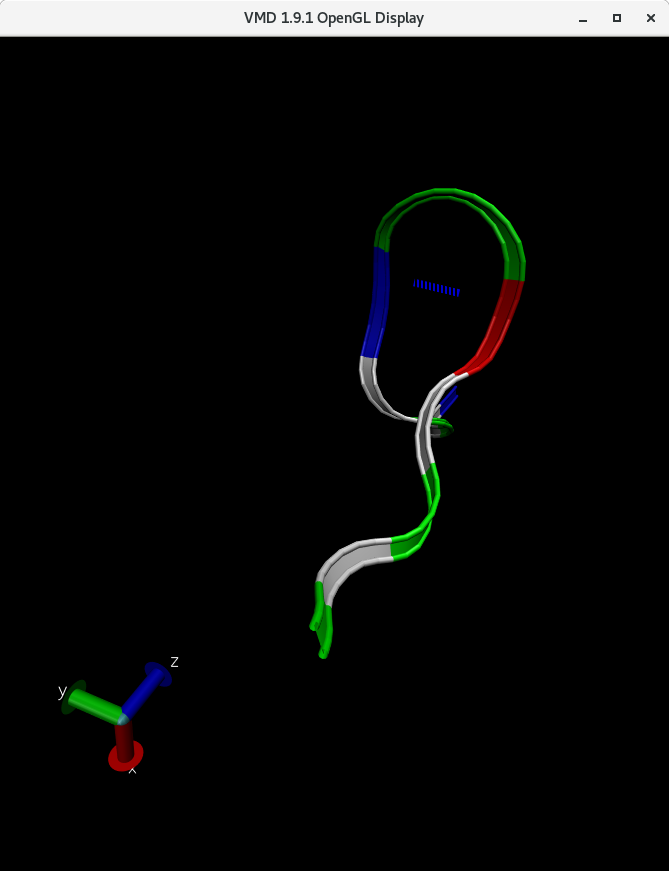
\includegraphics[scale=0.2]{HB}
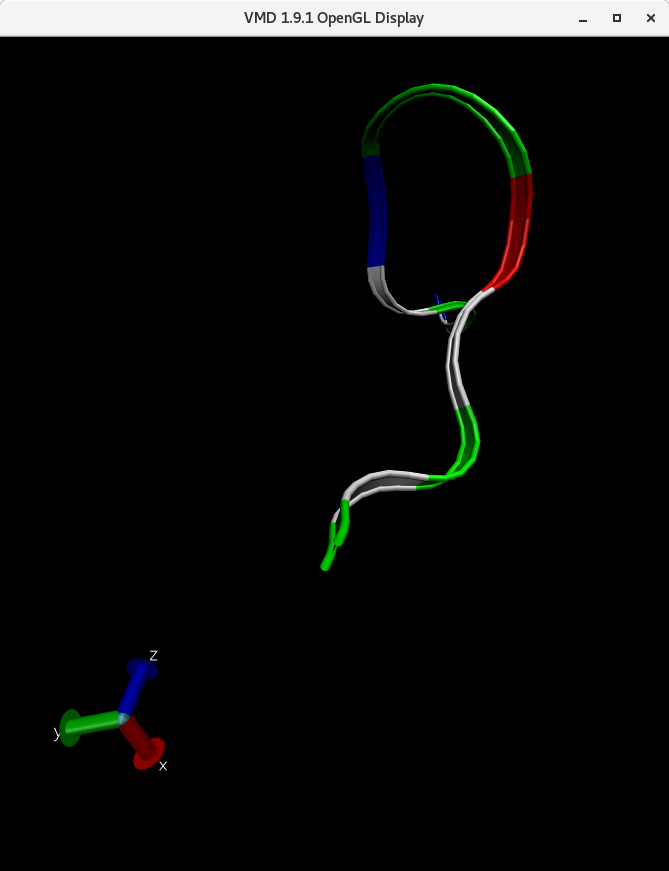
\includegraphics[scale=0.2]{NoHB}
\label{fig: hbondbye}
\caption{The hairpin in windows 10 and 11 (left, right).  The additional blue line (in the left figure) between the two sides of the hairpin represents a hydrogen bond and is not present in the right.}  
\end{figure}

The breaking of the hydrogen bond between these two structures is a possible cause of the change in shape of the PMF.  It also might explains why histograms 9 and 10 have such a large overlap.  If the potential barrier associated with this bond breaking was large enough then the bias potential in window 10 may not have been enough to maintain the reaction coordinate at a value of $z$ which coincided with the barrier.

\section{Conclusions}

We have shown the results of umbrella sampling simulations carried out on two simple proteins, a helix structure and a hairpin.  We have used WHAM to calculated the PMF from the umbrella histograms and used Bayesian bootstrapping to approximate the uncertainty in the calculated PMF.  For both structures the calculated PMF appeared to show some discontinuous behaviour.  We made an effort to characterise these \textit{spikes} and to explain them by investigating the overlap of the umbrella histograms.  We were able to find that the locations of the spikes coincided with significant under sampling and lack of overlap.  By characterising the overlap we were also to able to identify a potential cause for the change in nature of the PMF in the hairpin.  Further work could explore whether the other features that we identified were accompanied by a change in the structure of the proteins or were fully caused by the lack of sampling.\\

The pulling simulations of the helix were also analysed.  We were able to show that for slow pulling speeds the dominant effect on the force required is one of noise although we did not go into detail to explain why this was the case.

\begin{thebibliography}{}

\bibitem{StretchWhy} Strick, T. R., et al. "Stretching of macromolecules and proteins." Reports on Progress in Physics 66.1 (2002): 1.

\bibitem{Chig}Satoh, Daisuke, et al. "Folding free‐energy landscape of a 10‐residue mini‐protein, chignolin." FEBS letters 580.14 (2006): 3422-3426.

\bibitem{MDWhy} Rohs, Remo, Catherine Etchebest, and Richard Lavery. "Unraveling proteins: a molecular mechanics study." Biophysical journal 76.5 (1999): 2760-2768.

\bibitem{Umbrella} Kästner, Johannes. "Umbrella sampling." Wiley Interdisciplinary Reviews: Computational Molecular Science 1.6 (2011): 932-942.

\bibitem{PMF} Wong, Kin-Yiu, and Darrin M. York. "Exact relation between potential of mean force and free-energy profile." Journal of chemical theory and computation 8.11 (2012): 3998-4003.

\bibitem{GWHAM} Hub, Jochen S., Bert L. De Groot, and David Van Der Spoel. "g{\_}wham A Free Weighted Histogram Analysis Implementation Including Robust Error and Autocorrelation Estimates." Journal of chemical theory and computation 6.12 (2010): 3713-3720.

\bibitem{GMX} Lindahl, Abraham, Hess, \& van der Spoel. (2019, June 14). GROMACS 2019.3 Manual (Version 2019.3). Zenodo. http://doi.org/10.5281/zenodo.3243834

\bibitem{FF} Oostenbrink, Chris, et al. "A biomolecular force field based on the free enthalpy of hydration and solvation: the GROMOS force‐field parameter sets 53A5 and 53A6." Journal of computational chemistry 25.13 (2004): 1656-1676.

\bibitem{Ber} Lemak, A. S., and N. K. Balabaev. "On the Berendsen thermostat." Molecular Simulation 13.3 (1994): 177-187.

\bibitem{Jar} Jarzynski, Christopher. "Nonequilibrium equality for free energy differences." Physical Review Letters 78.14 (1997): 2690.

\bibitem{NH}
Martyna, Glenn J., Michael L. Klein, and Mark Tuckerman. "Nosé–Hoover chains: The canonical ensemble via continuous dynamics." The Journal of chemical physics 97.4 (1992): 2635-2643.

\bibitem{PR} Parrinello, Michele, and Aneesur Rahman. "Polymorphic transitions in single crystals: A new molecular dynamics method." Journal of Applied physics 52.12 (1981): 7182-7190.

\bibitem{VMD} Humphrey, W., Dalke, A. and Schulten, K., "VMD - Visual Molecular Dynamics", J. Molec. Graphics, 1996, vol. 14, pp. 33-38.

\bibitem{Rgyr} Lobanov, M. Yu, N. S. Bogatyreva, and O. V. Galzitskaya. "Radius of gyration as an indicator of protein structure compactness." Molecular Biology 42.4 (2008): 623-628.

\bibitem{IdCh} Rubinstein, Michael, and Ralph H. Colby. Polymer physics. Vol. 23. New York: Oxford university press, 2003.

\bibitem{Over} Swain, M. J., and D. H. Ballard. "Color Indexing International Journal of Computer Vision 7." (1991): 11-32.

\end{thebibliography} 

\end{document}